\documentclass[a4paper,11pt,twoside]{article}

\usepackage[utf8]{inputenc}
\usepackage[T1]{fontenc}
\usepackage[french]{babel}
	\frenchbsetup{SmallCapsFigTabCaptions=false}
\usepackage{indentfirst}
\usepackage[margin=2cm]{geometry}
\usepackage[table,kerneldraw,dvipsnames]{xcolor}
\usepackage{pdflscape}
\usepackage{rotating}

\usepackage{csquotes}
\usepackage[natbib=true,backend=biber,style=ieee,sort=none,sortcites=true,backref=true,backref=false,url=false,isbn=true,doi=true]{biblatex}
    \DefineBibliographyExtras{french}{\restorecommand\mkbibnamefamily}
    \AtBeginBibliography{\small}
    \addbibresource{references.bib}

\usepackage{fancyhdr}
\pagestyle{fancy}
\fancyhead{}
\fancyhead[C]{\textit{A. Huat / Projet de \DL\ (2018)}}
\fancyhead[LE,RO]{\thepage}
\fancyfoot{}
\renewcommand{\headrulewidth}{0pt}

\usepackage[nopostdot,nonumberlist,toc,acronyms]{glossaries}
\renewcommand{\glossarypreamble}{\small}

\usepackage{booktabs,array,longtable,tabularx}

\usepackage{menukeys}
\usepackage[shortcuts]{extdash}
\usepackage{enumitem}
%	\setlist{itemsep=0ex}
\usepackage{multicol}
\newenvironment{colfig}{\par\medskip\noindent\minipage{\linewidth}}{\endminipage\par\medskip}

\usepackage{float,here,placeins,graphicx,wrapfig}
	% Centering figures by default
	\makeatletter
	\g@addto@macro\@floatboxreset{\centering}
	\makeatother
\usepackage{}
\usepackage[labelfont=bf,justification=justified,font=small,labelsep=quad,tablename=Tableau]{caption}
	\floatplacement{figure}{htbp}
	\floatplacement{table}{htbp}

\usepackage[colorlinks=true,plainpages=false,breaklinks=true,allcolors=ProcessBlue]{hyperref}
\usepackage{fancyref}

\usepackage[newfloat]{minted}
    \newcommand{\listingautorefname}{Listing}
    \SetupFloatingEnvironment{listing}{name=Listing}
    \captionsetup[listing]{singlelinecheck=false}
    \usemintedstyle{friendly}
    \definecolor{grey05}{rgb}{0.95,0.95,0.95}
    \setminted{tabsize=4,fontsize=\footenotesize,frame=none,breaklines,bgcolor=grey05}

% Maths

\usepackage{cool}
\usepackage{upgreek}
\usepackage{upref}
\usepackage{mathtools}
\usepackage{amsmath}
\usepackage{amsfonts}
\usepackage{amsthm}
\theoremstyle{definition}
\usepackage{amssymb}
\usepackage[scaled=1.]{rsfso}
\usepackage[scaled=1.,mathscr]{urwchancal}
\usepackage{stmaryrd}

% --------------------------------------
% Macros
% --------------------------------------

\newcommand{\fnhref}[2]{\href{#1}{#2}\footnote{\url{#1}}}

\newcommand{\TODO}[1]{{\color{orange}\sffamily\textbf{TODO}\quad#1}}

\newcommand{\cad}{c'est-à-dire}
\newcommand{\Cad}{C'est-à-dire}
\newcommand{\pex}{par exemple}
\newcommand{\Pex}{Par exemple}
\newcommand{\AH}{Alexandre Huat}
\newcommand{\eg}{\textit{e.g.}}
\newcommand{\ie}{\textit{i.e.}}
\newcommand{\Ie}{\textit{I.e.}}
\newcommand{\etc}{\textit{etc.}}
\newcommand{\etal}{\textit{et al.}}
\newcommand{\vs}{\textit{vs.}}
\newcommand{\cf}{\textit{cf.}}
\newcommand{\Cf}{\textit{Cf.}}
\newcommand{\idem}{\textit{idem}}
\newcommand{\Idem}{\textit{Idem}}
\newcommand{\ibid}{\textit{ibid}}
\newcommand{\Ibid}{\textit{Ibid}}

\newcommand{\DL}{Deep Learning}
\renewcommand{\thefootnote}{\textit{\alph{footnote}}}

% Maths

% --------------------------------------
% Glossaire
% --------------------------------------

\makeglossaries

%%% Acronyms

\newacronym{eddp}{$(\epsilon, \delta)$-DP}{$(\epsilon, \delta)$--différentiellement confidentiel}

%%% Maths

% --------------------------------------
% Title
% --------------------------------------

\title{\textbf{Projet de \DL}\\«~Differentially Private Releasing via Deep Generative Model~»}
\author{\textbf{\AH}\\INSA Rouen Normandie\\Master Sciences et Ingénierie des Données}
\date{21 mars 2018}

% ======================================

\begin{document}
\maketitle
\thispagestyle{empty}

\part{Résumé d'article}
\label{resume}

Supposons un groupe de clients et un prestateur de services informatiques collectant et analysant leurs données (\eg\ classification d'images). Au cours des tâches d'analyses, le prestateur est amené à traiter des données sensibles. Afin de respecter la vie privée de ses clients, il doit trouver un moyen de traiter efficacement ces données tout en conservant leur confidentialité. C'est à cette problématique que répondent \citet{dpgan} par l'architecture dp-GAN de l'article résumé ici.

La \autoref{dp-gan_role} illustre le rôle de dp-GAN, qui est de générer des données synthétiques mais sémantiquement riches, \ie\ suffisamment représentatives des clients, sans violation de leur vie privée.
En introduction, les auteurs rappellent les défis à relever en apprentissage sous contrainte de confidentialité et présentent les apports de dp-GAN. En plus de sa capacité à générer une infinité de données, dp-GAN garantit l'anonymisation des données réelles par respect du principe de « confidentialité différentielle »\footnote{Synthétiqument, la confidentialité différentielle mesure la capacité d'un tiers à déduire des données privées des résultats d'un algorithme ; \cf\ exemple à \url{https://fr.wikipedia.org/wiki/Confidentialité_différentielle#Formalisation}.}.
Pour ce faire, dp-GAN applique au réseau adverse génératif de Wisserstein (WGAN) amélioré des mécanismes d'anonymisation à l'état de l'art, alors optimisés pour gagner en stabilité et en scalabilité.

\begin{figure}
    \centering
    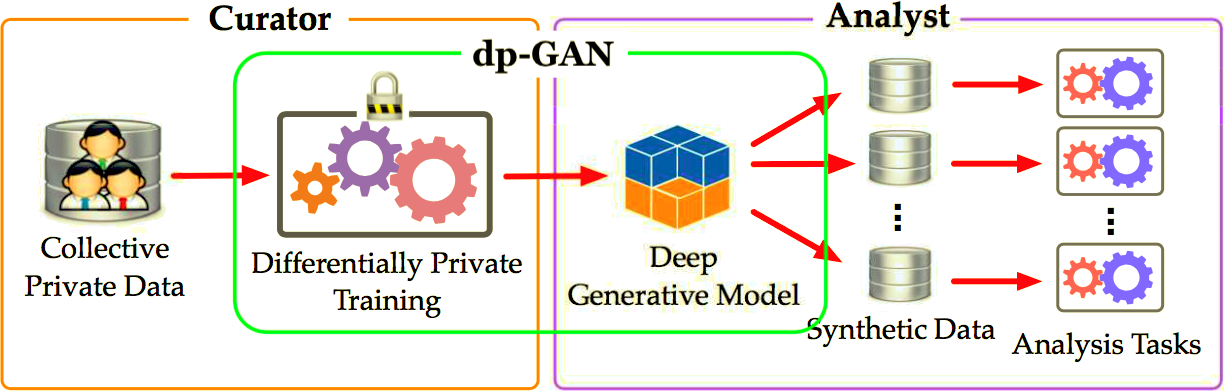
\includegraphics[width=12cm]{dp-gan_role.png}
    \captionof{figure}{La place de dp-GAN dans la chaîne de traitement des données confidentielles. Le « \textit{curator} » est l'entité qui anonymise les données pour l'\textit{analyst}.}
    \label{dp-gan_role}
\end{figure}

En Section 2, Zhang \etal\ font un rappel théorique sur les GAN et justifient leur utilisation du WGAN amélioré par une plus grande stabilité et un plus court temps d'apprentissage que le GAN origineligne Ils font également la définition formelle de la confidentialité différentielle et citent des propriétés associées dont bénéficient dp-GAN. La Section 3 présente dp-GAN dans sa version basique et fournit son algorithme d'apprentissage (Algorithme 1). Pour assurer sa confidentialité, à chaque mise-à-jour, l'algorithme bruite le gradient du discriminateur (bruitage gaussien et seuillage), à partir duquel un pirate pourrait autrement reconstruire les données privées. Cette technique est communément utilisée dans la littérature. Une preuve théorique du niveau de confidentialité différentielle atteint par l'algorithme est également apportée.

Néanmoins, cette version de dp-GAN possède trois inconvénients : (i) elle génère des données de faible qualité ; (ii) elle converge moins rapidement que le GAN non-confidentiel, voire diverge ; (iii) elle est rigide et n'exploite aucune ressource bonus, \eg\ des données publiques. Pour palier ces défauts, la version avancée de dp-GAN implémente : (i) un regroupement des paramètres du réseau pour un réglage fin et spécifique de leurs bruits respectifs ; (ii) un seuillage adaptatif du gradient, qui évolue au cours des itérations ; (iii) une initialisation des paramètres du réseau par pré-apprentissage sur les données publiques disponibles. Ces améliorations boostent la vitesse de convergence et la confidentialité de dp-GAN. La Section 4 détaille l'algorithme de  cette version avancée (Algorithme 3).

S'en suit un rapport d'expériences sur trois bases célèbres et libres d'accès : \href{http://yann.lecun.com/exdb/mnist/}{MNIST}, \href{http://mmlab.ie.cuhk.edu.hk/projects/CelebA.html}{CelebA} et \href{http://lsun.cs.princeton.edu/2015.html}{LSUN}. LSUN est ensuite divisée en deux bases, l'une labellisée (LSUN-L) et l'autre non-labellisée (LSUN-U). Les expériences sont réalisées avec TensorFlow (TF) mais le code n'est pas partagé par ses auteurs. Certains paramètres de tests sont renseignés mais l'architecture des réseaux générateurs et discriminateurs ne le sont pas. Ainsi, la Section 5 propose une évaluation qualitative et quantitative des performances du système. De mon point de vue, les images générées par dp-GAN, quelle que soit la base, sont assez vraisemblables ; MNIST en particulier est très bien simulée.
Dans leur deux premières expériences, Zhang \etal\ comparent quantitativement la qualité des données générées par dp-GAN aux données réelles et à celles générées par le GAN non-confidentieligne dp-GAN performe légèrement moins bien pour les données labellisées comme pour les non-labellisées. Dans leur troisième expérience, les auteurs comparent les performances atteintes en classification sur LSUN-L après apprentissage sur : (i) les données réelles seules ; (ii) les données réelles jointes aux données synthétisées par un GAN non-confidentiel ; (iii) les données réelles jointes aux données synthétisées par dp-GAN. Il en ressort que l'apprentissage avec les données synthétiques permet systématiquement une diminution des taux d'erreurs (jusqu'à $-3.3 \%$ pour dp-GAN, contre $-7.7 \%$ pour le GAN non-confidentiel). Quatrièmement, en terme de score d'Inception et de Jensen-Schannon, une ultime expérimentation valide l'efficacité des stratégies d'optimisations dont bénéficie dp-GAN avancé.

Dernièrement, les auteurs consacrent une section aux travaux similaires de la littérature. Puis, ils concluent en rappelant l'intérêt et les améliorations apportées par dp-GAN et, enfin, ouvrent la discussion sur la limite que l'architecture n'a été testée que sur des images -- une évaluation sur d'autres types de données (\eg\ texte) étant bienvenue.

\part{Implémentation}
\label{impl}

Cette partie détaille mon implémentation de dp-GAN, les difficultés rencontrées et les solutions développées. La \autoref{obj} définit les objectifs du projet. La \autoref{techno} rappelle l'algorithme de dp-GAN basique et présente la technologie utilisée pour son développement. En \autoref{code}, nous verrons plus précisément le code développé. Puis, des résultats de tests sont exposés en \autoref{res}, que la \autoref{conc} analyse avant de conclure.

\paragraph{Adresse}
Le projet est disponible sur Github à : \url{https://github.com/alexandrehuat/dp-gan}.


\section{Objectifs}
\label{obj}

Le véritable défi de ce projet, et en accord avec l'objet du cours de \DL, est l'implémentation de dp-GAN basique. En effet, celle-ci demande une prise en main de WGAN amélioré et des calculs de confidentialité différentielle \citep{dlwdp, pinq}. En comparaison, dp-GAN avancé ne consiste qu'en l'enrichissement de dp-GAN basique d'un apprentissage sur des données publiques et d'un \textit{clustering} hiérarchique des paramètres du réseau. Or, comptant ma formation en apprentissage statistique, ces opérations ne présentent pas de plus-value pédagogique. Sachant le temps allouable au projet, il m'est apparu raisonnable de me concentrer sur l'implémentation de dp-GAN basique. Quant aux données d'expérimentation, j'ai choisi la base MNIST pour faciliter l'apprentissage et l'interprétabilité des résultats.


\section{Algorithme, technologie et organisation}
\label{techno}

\begin{figure}
    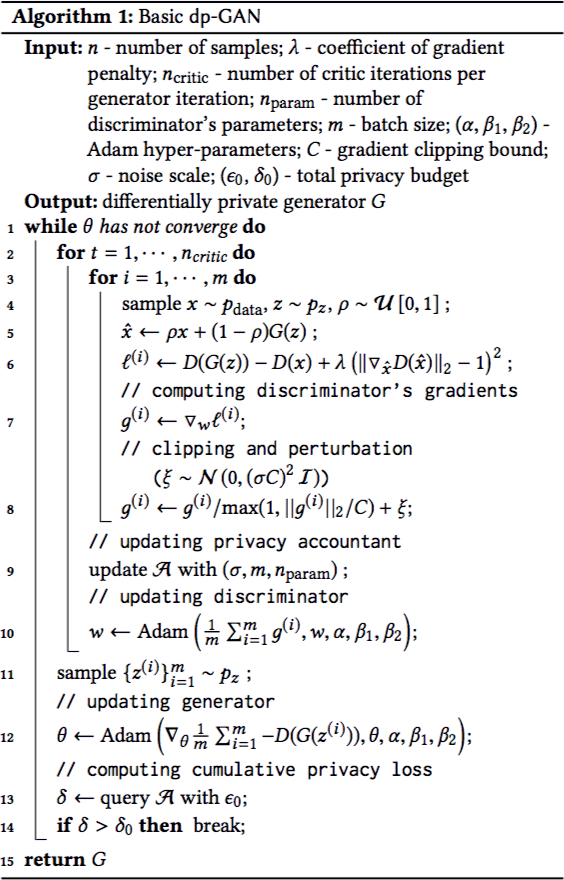
\includegraphics[width=10cm]{alg1.png}
\end{figure}

Comme dit en \autoref{resume}, l'algorithme d'apprentissage de dp-GAN basique (Algorithme 1) est celui de WGAN amélioré avec un bruitage et seuillage de gradients. Étant donné l'avènement de TF dans la communauté du \DL\ ainsi que l'utilisation de cette librairie par \citet{dpgan}, j'ai choisi de réaliser toute la partie bas niveau du projet (apprentissage de dp-GAN) en TF et d'utiliser Keras pour les opérations de plus haut niveau (création, sauvegarde et évaluation des modèles). L'utilisation de TF était nécessaire pour brouiller le gradient (Algorithme 1, ligne 8), en recherche de confidentialité. Sans ces opérations, le projet aurait essentiellement été une implémentation de WGAN amélioré\footnote{Implémentation totalement réalisable en Keras par alternance d'apprentissage du générateur $G$ et du discriminateur $D$ en gelant les poids de $G$ quand $D$ apprend, resp. de $D$ quand $G$ apprend.}. De plus, connaissant Keras par de précédents cours, projets personnels ou le PIC Becquerel 2017, un projet en Keras pur m'aurait donné plus de temps pour les tests ou l'amélioration de la méthode implémentée. À l'inverse, je ne connaissais pas TF avant ce projet, et dédiai donc au moins la moitié de mes efforts au développement de dp-GAN basique. Puis, je consacrai le temps restant au pré-apprentissage et au test des modèles. Je reviendrai sur ces points en \autoref{app} et \ref{res}. Bien sûr, je donnai également du temps à la rédaction de ce rapport.

Enfin, je dois préciser qu'il ne m'a pas été possible d'implémenter la partie « vérification de la confidentialité » de dp-GAN (Algorithme 1, ligne 9 et 13). En effet, les auteurs donnaient trop peu d'explications sur ces opérations et il m'aurait fallu lire \cite{dlwdp} et \cite{pinq} pour les intégrer. Si je me suis si facilement permis de l'omettre, c'est aussi parce cette partie sortait du cadre \Dligne Toutefois, son absence n'impacte pas l'apprentissage de dp-GAN en dehors du retrait d'un critère d'arrêt.


\section{Code}
\label{code}

Cette section explique le code du projet et se veut comme preuve de ma bonne implémentation de dp-GAN basique.

\subsection{Architecture générale}
Mon code de dp-GAN (fichier \texttt{dpgan/dpgan.py}) est plutôt concis puisqu'il consiste en deux classes: \mintinline{python}$DPGAN$ une classe abstraite dont les attributs sont les réseaux $G$ et $D$, et \mintinline{python}$BasicDPGAN$ une classe dérivée qui implémente la fonction d'apprentissage \mintinline{python}$train()$. Parcourons cette fonction, puisqu'elle est au cœur du projet.

Les paramètres de \mintinline{python}$train()$ sont:
\begin{description}
    \item[\mintinline{python}$X$] les données d'apprentissage
    \item[\mintinline{python}$epochs$] le nombre maximal d'itérations à réaliser si $G$ ne converge pas (Algorithme 1, boucle \textbf{while}). Pour dp-GAN, une \textit{epoch} n'est pas une passe entière du jeu de données, mais une passe de $(n_\mathit{critic}+1) \times m$ exemples.
    \item[\mintinline{python}$lam$] le coefficient de régularisation de WGAN amélioré
    \item[\mintinline{python}$n_critic$] le nombre de \textit{batch} vu par $D$ avant mise à jour de $G$
    \item[\mintinline{python}$batch_size$] la taille des \textit{batchs} d'apprentissage ($m$ dans l'Algorithme 1)
    \item[\mintinline{python}$optimizer$] l'optimiseur TF réalisant les descentes de gradients des deux réseaux
    \item[\mintinline{python}$C$] la borne de seuillage du gradient
    \item[\mintinline{python}$sigma$] un coefficient de variance du bruit gaussien appliqué au gradient de $D$
    \item[\mintinline{python}$eps0, delta0$] le budget de confidentialité\footnote{Inutilisé dans le projet.}
    \item[\mintinline{python}$tol$] le seuil de tolérance évaluant la convergence du gradient de $G$
    \item[\mintinline{python}$save_paths$] les chemins de sauvegarde progressive des modèles (pour permettre un redémarrage à froid)
\end{description}

Voyons maintenant son fonctionnement. \mintinline{python}$train()$ est divisée en deux parties « exigées » par TF:
\begin{enumerate}
    \item la définition d'opérations symboliques qu'effectueront les réseaux de neurones (le « \textit{tensor flow} »);
    \item l'exécution des calculs (j'y compte l'initialisation des variables et l'exécution de l'apprentissage).
\end{enumerate}

La première partie fut la plus complexe, car elle demande une bonne maîtrise de TF et une bonne compréhension de ses structures. La classe centrale de TF est \mintinline{python}$tf.Tensor$, une implémentation de l'objet mathématique généralisant les matrices et les vecteurs. Dans la plupart des cas, les \mintinline{python}$tf.Tensor$ manipulés sont de dimension \mintinline{python}$(batch_size, N, M, ...)$ où \mintinline{python}$N, M, ...$ sont les dimensions des données, de variables diverses (\eg\ poids et biais) ou de gradients. Dans ma première implémentation, j'essayai d'utiliser des tenseurs de taille \mintinline{python}$(N, M, ...)$ mais cela ne marchait pas bien, et, dans la documentation, il est recommandé d'utiliser les tenseurs comme mentionné juste avant. De plus, réaliser les boucles sur les \textit{batch} de données directement par TF rendait mon code plus rapide. J'adaptais donc mon code, ce qui me demanda assez de travail. Comme variables clés de la fonction \mintinline{python}$train()$, on trouve:
\begin{description}
    \item[\mintinline{python}$D_loss$] un tenseur, qui correspond à la moyenne d'un \textit{batch} de $\ell^{(i)}$ (Algorithme 1, ligne 6).
    \item[\mintinline{python}$D_grad_vars$] une liste de tuples \mintinline{python}$(grad, var)$, où pour le $l$-ième tuple, \mintinline{python}$grad$ correspond à la moyenne d'un \textit{batch} de gradients $g^{(i)}$ (lignes 7 et 8) par rapport à \mintinline{python}$var$ les paramètres de la $l$-ième couche de $D$.
    \item[\mintinline{python}$G_loss$] un tenseur, qui correspond au coût $\frac{1}{m} \sum_{i=1}^m -D(G(z^{(i)}))$ que $G$ minimize (ligne 12).
\end{description}

Une fois ces tenseurs et les opérations de minimisations déclarées, ces dernières sont trivialement exécutées par une session TF dans les boucles \textbf{for} appropriées.

\paragraph{Remarque} Dans l'Algorithme 1, $g^{(i)}$ se voit appliquer un bruit gaussien $\xi$ d'espérance 0 et d'écart type $\sigma C$\footnote{Par élément, car la matrice de covariance de $\xi$ est $(\sigma C)^2 \mathbf{I}$ où $\mathbf{I}$ est la matrice identité de même dimension que $g^{(i)}$.} à chaque $i$-ème exemple d'un \textit{batch} (ligne 8). Puis, Adam descend la moyenne de ces gradients. Mais, dans mon implémentation, la moyenne des gradients est calculée avant l'ajout de $\xi$. Toutefois, ceci reste valide, car, par application du théorème centrale limite, la moyenne des $\xi$ converge en loi vers $\xi$.


\subsection{Descente de gradient}

Pour la descente de gradients, j'eu à apprendre le fonctionnement des optimiseurs de TF. Dans le cas basique, il suffit d'utiliser la méthode \mintinline{python}$minimize(loss, var_list=<weights>, ...)$ de la classe \mintinline{python}$tf.train.Optimizer$ pour optimiser les paramètres d'un réseau en fonction d'un coût. Mais dp-GAN nécéssite des opérations intermédiaires sur le gradient. J'utilise donc \mintinline{python}$compute_gradients(loss, var_list, ...)$ dont je modifie le résultat avant d'optimiser les paramètres avec \mintinline{python}$apply_gradients(grad_and_vars, ...)$.
Ainsi, mon implémentation permet l'apprentissage de dp-GAN avec n'importe quel optimiseur TF.


\subsection{Interfaçage de TF et Keras}
\label{tf_keras}

De manière générale, l'interfaçage de TF et Keras est fluide, presque transparent. Cependant, j'ai rencontré une difficulté lorsque je souhaitais évaluer les réseaux via Keras après leur apprentissage avec TF. En effet, j'obtenais une erreur du type:
\mint{python}$FailedPreconditionError: Attempting to use uninitialized value <layer_name>/bias$
Cette erreur était causée par la perte de la référence des poids des réseaux après l'apprentissage. Ceci car les poids dépendent de la session TF qui les mets à jour, et que cette session était éphémère dans ma première implémentation. Ainsi, j'ai résolu ce problème en pérénisant la session sous la forme d'un attribut de \mintinline{python}$DPGAN$ (\cf\ \autoref{tfsess_after}) plutôt que d'utiliser une session locale à la fonction d'apprentissage (\cf\ \autoref{tfsess_before}).

\begin{listing}
\caption{Gestion des sessions TF avec erreur}
\label{tfsess_before}
\begin{minted}{python}
def BasicDPGAN(DPGAN):
    def train(...):
        ...  # Préparation des calculs
        with tf.Session() as sess:
            <results> = sess.run(<training>)  # Exécution des calculs
        return <results>  # La référence est supprimée à ce moment
\end{minted}
\end{listing}

\begin{listing}
\caption{Gestion des sessions TF sans erreur}
\label{tfsess_after}
\begin{minted}{python}
def BasicDPGAN(DPGAN):
    def train(...):
        ...  # Préparation des calculs
        <results> = self.tf_session.run(<training>)  # Exécution des calculs
        self.tf_session.close()
        return <results>
\end{minted}
\end{listing}


\section{Apprentissage}
\label{app}

L'apprentissage de dp-GAN est une procédure fastidieuse et dure à paramétrer. Dans \cite{dpgan}, les auteurs ne précisent ni les architectures neuronales utilisées sur les réseaux, ni le paramètre de seuillage $C$. Pour les calculs, mon compte Multipass ne me permettait pas de me connecter au GPU. J'utilisai alors ma machine personnelle, un Macbook Air avec macOS High Sierra, un processeur à deux cœurs Intel Core i7 @ 2.2 GHz et une RAM de 8 GO @ 1600 MHz. Ceci me contraint d'utiliser de petites architectures peu profondes détaillées ci-dessous (couches cachées uniquement).

\begin{description}
    \item[Générateur] Auto-encodeur à 3 couches denses (89, 10 et 89 neurones).
    \item[Discriminateur] CNN à 3 couches convolutionnelles de 64 neurones alternées de couches de \textit{max pooling}, et terminé par 2 couches denses de 512 neurones.
\end{description}

J'ai utilisé la fonction d'activation SELU pour les couches cachées des réseaux, car elle leur donne des propriétés auto-normalisantes et a donné de bonnes performances dans la littérature \cite{selu}.

\paragraph{Test 0}
Dans un premier temps, j'ai essayé d'apprendre directement mes réseaux avec dp-GAN, mais les résultats étaient médiocres. À titre d'illustration, la \autoref{fig:loss_bad_dpgan_nop} montre un apprentissage (d'une heure) qui diverge à partir d'un nombre d'\textit{epochs} insuffisant pour entraîner $G$ à produire des images réalistes (comme l'atteste la \autoref{fig:im_bad_dpgan_nop}). Par conséquent, j'ai choisi d'améliorer mes expériences d'un pré-apprentissage séparé des réseaux suivi d'une optimisation fine avec dp-GAN.

\begin{figure}
    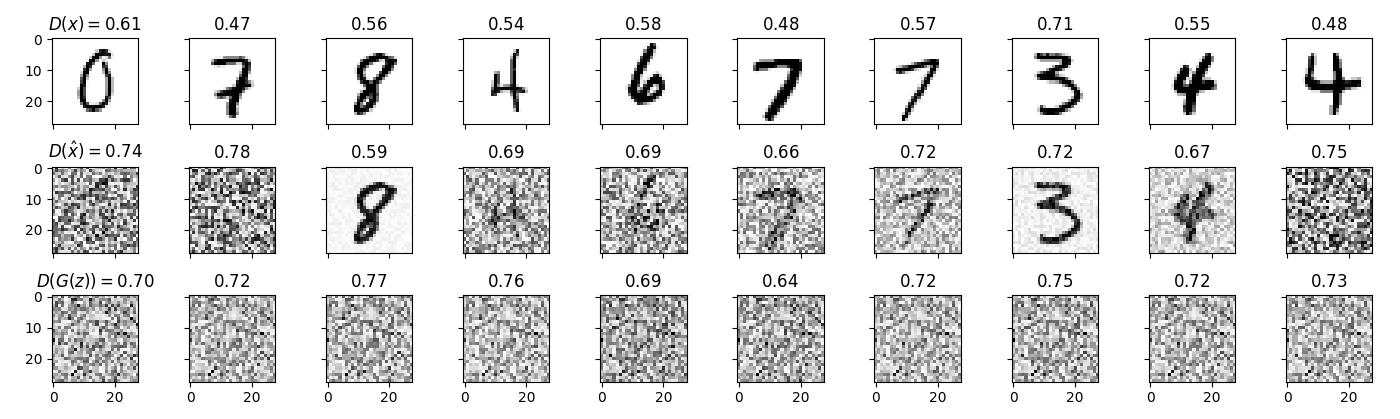
\includegraphics[width=\linewidth]{test0im.png}
    \caption{Exemples de données générées par $G$ à l'issue du test 0. La ligne du haut est celle des vraies images, la ligne du milieu est celle d'images bruitées et la ligne du bas est celle d'images générées par dp-GAN. Le titre de chaque image mesure le réalisme que lui attribue $D$. Les images générées par dp-GAN ne ressemblent en rien à des chiffres, mais forment toutefois un motif spécifique, que $D$ trouve plus vraisemblable que les images réelles. Des images similaires sont obtenues tout au long de l'apprentissage.}
    \label{fig:im_bad_dpgan_nop}
\end{figure}

\begin{figure}
    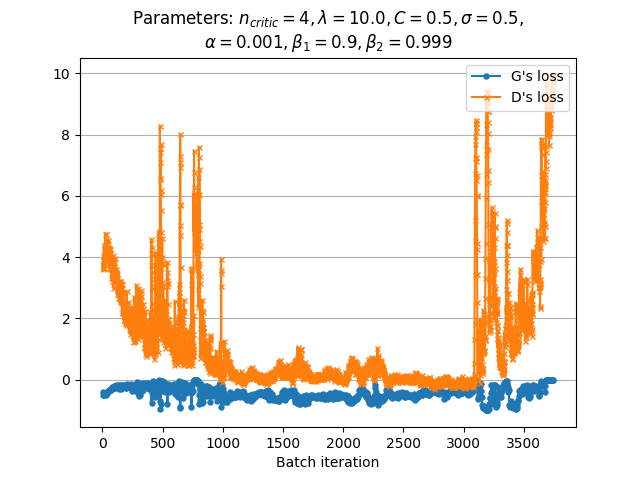
\includegraphics[width=0.6\linewidth]{test0loss.png}
    \caption{Évolution des coûts de dp-GAN en fonction du nombre d'\textit{epochs}. Passé 3000 \textit{batchs} ($= \frac{64 \times 3000}{60000} = 3.2$ fois la base d'apprentissage), $D$ diverge.}
    \label{fig:loss_bad_dpgan_nop}
\end{figure}

\section{Résultats}
\label{res}

Cette section présente les résultats de mes expériences. Je ne présente que peu de figures, les plus représentatives, car comme mentionné dans les sections précédentes, j'ai concentré mon temps sur l'implémentation de dp-GAN.

\subsection{Pré-apprentissage {\normalfont(Fichier \texttt{dpgan/pretrain.py})}} Pour améliorer l'apprentissage sous dp-GAN, j'ai réalisé un pré-apprentissage de $G$ avec comme coût l'erreur quadratique moyenne (MSE) et comme optimiseur Adam (paramétré par défaut par Keras). J'ai ainsi amené $G$ à 0.0297 de MSE de test en 50 \textit{epochs}, au-delà desquelles il aurait surappris. Les Figures \ref{fig:pretrain_g_30} et \ref{fig:pretrain_g_50} illustrent les résultats de ce pré-apprentissage.

Pour $D$, j'ai entraîné le réseau à classifier MNIST, l'amenant à 1.89 \% de taux d'erreur en 2 \textit{epochs}. Évidemment, à ce moment la couche de sortie était une couche dense de 10 neurones activés par une fonction $\mathrm{softmax}$. Mais lors de l'apprentissage de dp-GAN, j'ai changé la couche de sortie de $D$ en une couche dense d'un seul neurone, activé par la fonction sigmoïde pour obtenir une probabilité que la donnée entrée soit vraie. Le principe du pré-apprentissage était de faire du \textit{transfert learning} des couches convolutionnelles, alors gelées durant l'apprentissage de dp-GAN.

\begin{figure}
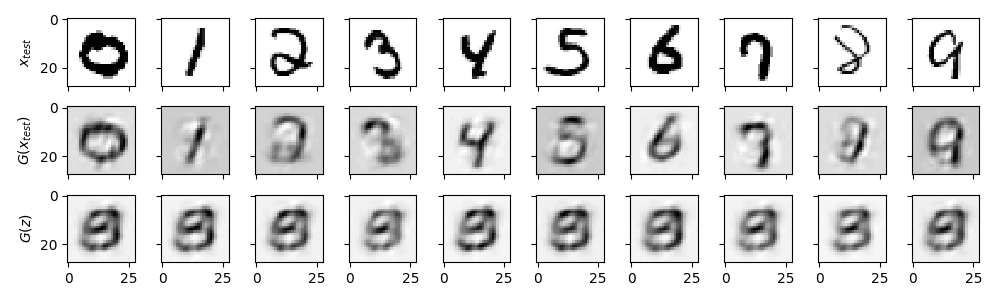
\includegraphics[width=\linewidth]{pretraining_G_30epochs.png}
\caption{Exemples de données générées par $G$ après 30 \textit{epochs} de pré-apprentissage. La ligne du haut représente des vrais exemples de tests, la ligne du milieu les mêmes exemples reconstruits et la ligne du bas des exemples générés à partir d'un bruit uniforme. On voit que $G$ a encore un peu de mal à reconstruire le 2 et le 8, par exemple.}
\label{fig:pretrain_g_30}
\end{figure}

\begin{figure}
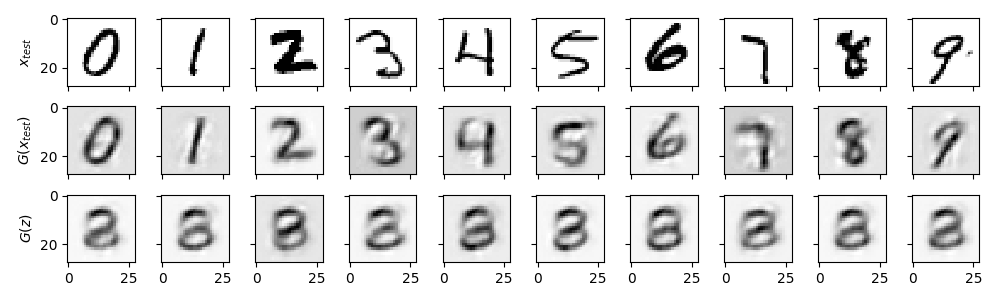
\includegraphics[width=\linewidth]{pretraining_G_50epochs.png}
\caption{Exemples de données générées par $G$ après 50 \textit{epochs} de pré-apprentissage. La ligne du haut représente des vrais exemples de tests, la ligne du milieu les mêmes exemples reconstruits et la ligne du bas des exemples générés à partir d'un bruit uniforme. À ce niveau, $G$ reconstruit très bien les images, si ce n'est le fond toujours grisâtre plutôt que blanc.}
\label{fig:pretrain_g_50}
\end{figure}

\subsection{Tests de dp-GAN {\normalfont(Fichier \texttt{dpgan/tests.py})}}
À titre d'exemple, voyons maintenant deux résultats distincts d'apprentissage de dp-GAN.

\paragraph{Test 1}
Dans un premier temps, j'ai entraîné dp-GAN pendant 1000 \textit{epochs} (30 minutes), avec les mêmes paramètres que ceux utilisés par ses auteurs, précisés en Tableau 1 de \cite{dpgan}. La \autoref{fig:loss_bad_dpgan} illustre l'évolution du côut des réseaux au cours des \textit{epochs} et la \autoref{fig:im_bad_dpgan} les images que $G$ génère. On voit que $D$ et $G$ n'apprennent pas avec ces paramètres, pour lesquelles les coûts divergent resp. sont instables.

\begin{figure}
    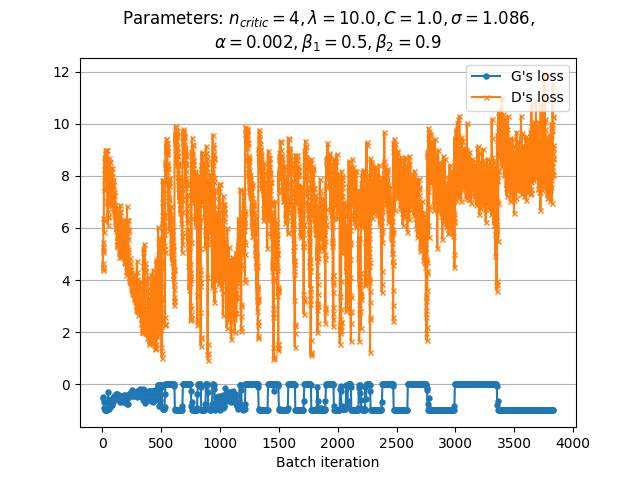
\includegraphics[width=0.6\linewidth]{test1loss.png}
    \caption{Évolution du coût de dp-GAN en fonction du nombre d'\textit{epochs} dans le test 1}
    \label{fig:loss_bad_dpgan}
\end{figure}

\begin{figure}
    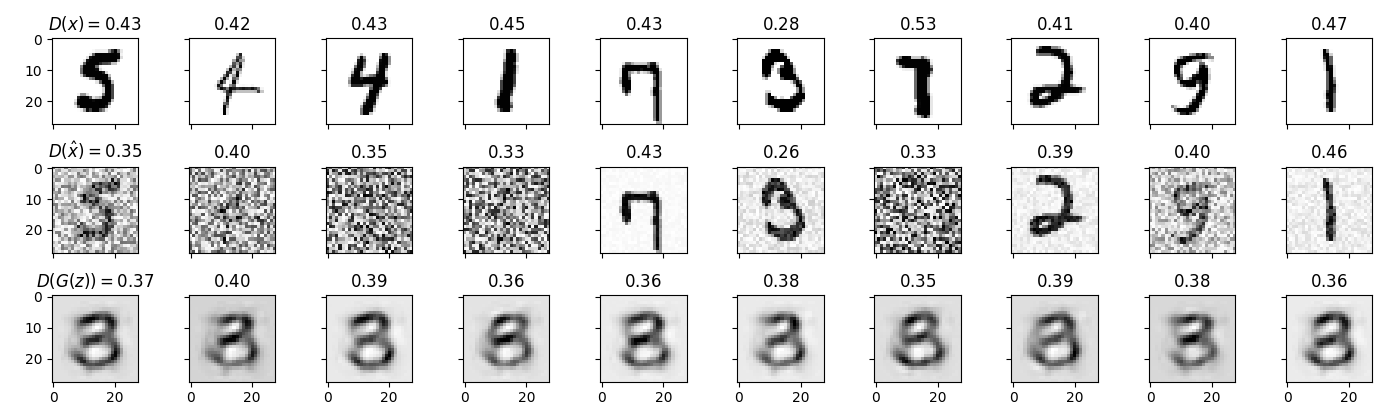
\includegraphics[width=\linewidth]{test1im.png}
    \caption{Exemple d'images générées par dp-GAN après l'apprentissage du test 1. Le titre de chaque image indique la probabilité que l'image soit vraie selon $D$. La ligne du haut est celle des vraies images, la ligne du milieu est celle d'images bruitées et la ligne du bas est celle d'images générées par dp-GAN.}
    \label{fig:im_bad_dpgan}
\end{figure}

\paragraph{Test 2}
Dans un deuxième temps, j'ai entraîné dp-GAN pendant 1000 \textit{epochs} (30 minutes), avec les paramètres précisés en figure \autoref{fig:loss_good_dpgan}. (En particulier, les paramètres d'Adam sont ceux par défaut de Keras.) On constate une meilleure descente de gradient qu'en test 1 pour $D$ (\cf\ \autoref{fig:loss_good_dpgan}). $G$ ne change pas vraiment, mais les images .

\begin{figure}
    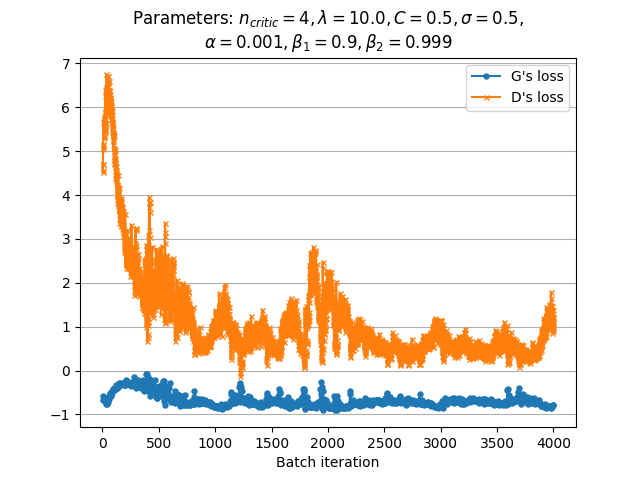
\includegraphics[width=0.6\linewidth]{test2loss.png}
    \caption{Évolution du coût de dp-GAN en fonction du nombre d'\textit{epochs} dans le test 2}
    \label{fig:loss_good_dpgan}
\end{figure}

\begin{figure}
    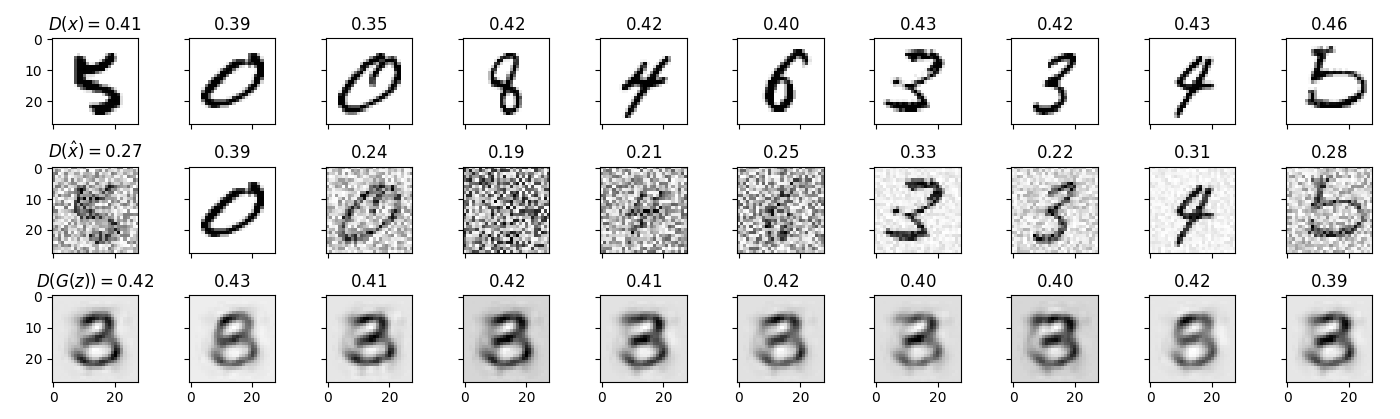
\includegraphics[width=\linewidth]{test2im.png}
    \caption{Exemple d'images générées par dp-GAN après l'apprentissage du test 2. Le titre de chaque image indique la probabilité que l'image soit vraie selon $D$. La ligne du haut est celle des vraies images, la ligne du milieu est celle d'images bruitées et la ligne du bas est celle d'images générées par dp-GAN.}
    \label{fig:im_good_dpgan}
\end{figure}

\begin{table}
    \caption{Évaluation quantitative de $D$ après apprentissage par dp-GAN. $s_+ \in [0; 1]$ est le score de surestimation moyenne, tel que $s_+(\mathcal{X})= \frac{1}{\lvert \mathcal{X} \rvert} \sum_{x \in \mathcal{X}} (D(x)-y_x)$ où $\mathcal{X}$ est une base de données et $y_x = 1$ si $x$ est une vraie donnée, 0 sinon (si $x$ est du bruit ou une donnée générée). Plus $s_+$ est proche de 0, meilleur est $D$.}
    \label{tab:eval_dpgan}
    \begin{tabular}{@{}lrrr@{}}
        \toprule
        \textbf{Critère} & \textbf{Test 0} & \textbf{Test 1} & \textbf{Test 2} \\ \midrule
        $s_+(X_\mathit{test})$ & -0.3215 & -0.5656 & -0.6026 \\
        $s_+(Z)$ & 0.5294 & 0.3814 & 0.2233 \\
        $s_+(G(Z))$ & 0.5137 & 0.3746 & 0.4133 \\
        \bottomrule
    \end{tabular}
\end{table}

Le \autoref{tab:eval_dpgan} montre que $D$ sous-estime largement les données réelles de tests. Dans les tests 0 et 1, $D$ ne fait pas de différence entre un bruit uniforme et une donnée générée par dp-GAN. Ce que suggère également les Figures \ref{fig:im_bad_dpgan_nop} et \ref{fig:im_bad_dpgan}. En revanche, dans le test 2, $D$ à atteint un équilibre probabiliste entre les données réelles et synthétiques ($\approx 40~\%$) et trouve le bruit deux fois moins réaliste que les images réelles ou synthétiques. Ce sont les seuls résultats encourageant.


\section{Discussion et conclusion}
\label{conc}

Tout d'abord, au regard de mes objectifs, le projet est une réussite. En effet, je suis parvenu à développer dp-GAN basique de zéro en utilisant TF, interfacé avec Keras, rendant possible l'apprentissage de n'importe quel couple de réseaux générateur et discriminateur, avec n'importe quel optimiseur TF.

Afin, d'évaluer mon travail, sur MNIST, j'ai d'abord tenté l'apprentissage d'un auto-encodeur $G$ couplé à un réseau convolutionnel $D$ via dp-GAN. Les résultats n'étant pas concluants, j'ai ensuite réalisé deux autres tests où je précédai l'apprentissage de dp-GAN de pré-apprentissages séparés de $D$ et $G$. Nous pouvons en faire les remarques suivantes. Premièrement, on constate peu de différences entre $G$ pré-appris et $G$ affiné avec dp-GAN. dp-GAN a essentiellement permis la spécification de $D$ sur la tâche de discrimination. Et si le coût $\frac{1}{m}\sum_{i=1}^m -D(G(z))$ minimisé par $G$ évolue, c'est probablement car $D$ évolue. Ceci peut être attribué au mauvais paramétrage de l'apprentissage. Le question des architectures se pose également ($G$ n'a que 3 couches cachées de 10 ou 89 neurones), mais je ne pense pas que cela soit une limite majeure. Nous pouvons également critiquer le choix de $Z$, la distribution des entrées de $G$. J'ai en effet utilisé une loi uniforme, car c'est ce qui est habituellement fait, et que la distribution $Z$ utilisée en \cite{dpgan} n'y est pas précisée. Or, l'on sait, et les figures des sections précédentes l'attestent, que l'entrée du réseau affecte profondément sa sortie, et donc le résultate de la rétro-prépogation du gradient pour l'apprentissage. Aussi, je n'ai entraîné dp-GAN que sur 1000 \textit{epochs} avec une taille de \textit{batch} de 64, contraint par l'instabilité de l'apprentissage et ma puissance machine. C'est très peu, considérant que cela correspond à une seule passe de MNIST. Enfin, si le test 2 aboutit à de meilleurs résultats que le test 1, c'est aussi hypothétiquement dû à un plus faible bruitage du gradient et un meilleur paramétrage d'Adam. Dernièrement, en réalité, un tel pré-apprentissage ne serait pas effectué sur dp-GAN, car la base de donnée est censée être privée. Il y a donc beaucoup d'éléments manquants dans la publication soumise par \citet{dpgan}, car les résultats qu'ils obtiennent sur MNIST sont incomparablement meilleurs que les miens.

En conclusion, même si je n'ai pas retrouvé les résultats de la publication originelle de dp-GAN, ce projet m'aura appris à utiliser TF pour des opérations de bas niveau sur les coûts et gradients de réseaux de neurones. Je me sens maintenant à l'aise avec TF, dont les structures m'apparaissent intuitives, et avec l'API fonctionnelle de Keras. Les objectifs du projet ont été atteint.


\printbibliography[title=Références,heading=bibintoc]
\end{document}
